\documentclass[11pt]{article}
\usepackage[a5paper,margin=14mm]{geometry}
\usepackage{fontspec}
\setmainfont{TeX Gyre Pagella}
\setsansfont{TeX Gyre Heros}
\usepackage{amsmath}
\usepackage{pgfplots}
\pgfplotsset{compat=1.18}
\usepgfplotslibrary{groupplots}

\begin{document}
\section*{Function plots}
\begin{center}
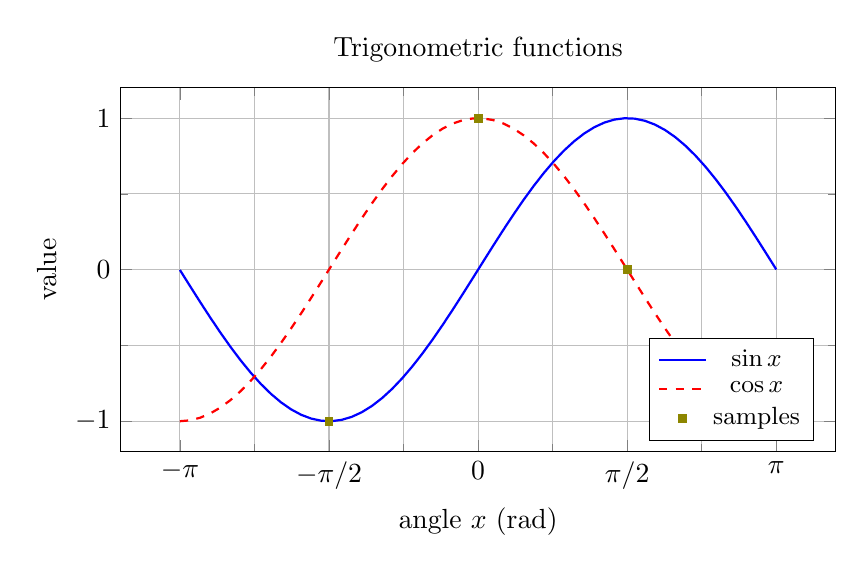
\begin{tikzpicture}
\begin{axis}[
  width=.88\linewidth,height=6.2cm,
  title={Trigonometric functions},
  xlabel={angle $x$ (rad)},ylabel={value},
  domain=-3.14:3.14,samples=60,
  legend pos=south east,legend style={font=\small},
  grid=both,minor tick num=1,
  xtick={-3.14,-1.57,0,1.57,3.14},
  xticklabels={$-\pi$,$-\pi/2$,$0$,$\pi/2$,$\pi$}]
  \addplot[blue,thick] {sin(deg(x))};
  \addlegendentry{$\sin x$}
  \addplot[red,thick,dashed] {cos(deg(x))};
  \addlegendentry{$\cos x$}
  \addplot[olive,only marks,mark=square*,mark size=1.4pt] coordinates {(-1.57,-1)(0,1)(1.57,0)};
  \addlegendentry{samples}
\end{axis}
\end{tikzpicture}
\end{center}

\begin{center}
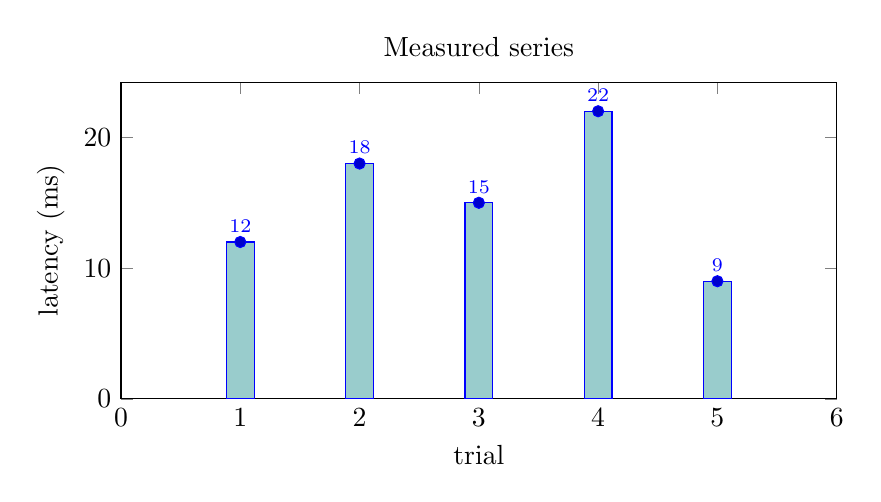
\begin{tikzpicture}
\begin{axis}[
  width=.88\linewidth,height=5.6cm,
  title={Measured series},
  xlabel={trial},ylabel={latency (ms)},
  xmin=0,xmax=6,ymin=0,
  nodes near coords,every node near coord/.append style={font=\scriptsize}]
  \addplot+[ybar,fill=teal!40] table[row sep=\\] {
    x y \\
    1 12 \\
    2 18 \\
    3 15 \\
    4 22 \\
    5 9 \\
  };
\end{axis}
\end{tikzpicture}
\end{center}
\end{document}
